\chapter{Complex Networks}
\label{cha:intro}

Networks constitute the backbone of any complex system
\cite{10.5555/3181286}, from the human brain to transport infrastructures, online social systems and financial markets. Characterising their structure and behaviour improves our understanding of the phenomena that shape the world we live in and its society. Complex networks are systems consisting of a high number of units (nodes) interconnected through highly non-trivial interaction patterns. The human brain, social systems, both on and off the Internet, are common examples of complex systems modelled through complex networks but other examples like water distribution, transport systems and blood flux show that complex networks are all around us and shape nearly everything we are surrounded with nowadays, from metabolic to online systems. One of the key features of complex networks is that they often exhibit a degree of clustering, meaning that nodes tend to be highly connected to other nodes that are nearby in the network. This can lead to the formation of small, tight communities within the larger network, i.e. social communities and friendship groups. Another important feature emerged from studies of complex networks \cite{articl2e} is that they often exhibit a power-law distribution of node degrees, meaning that there are relatively few highly connected nodes (hubs), and many more nodes with relatively few connections. On social networks, this is the case of influencers. This makes understanding complex networks extremely important and so are all the developments in this branch, whose results have been already proven to have a huge impact on practical disciplines.

\begin{center}
    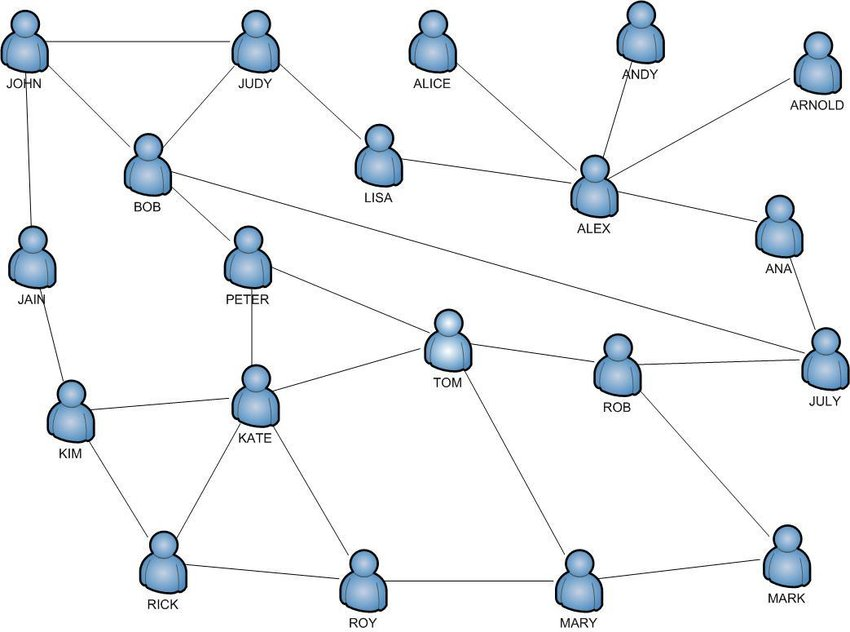
\includegraphics[scale=0.4]{complexnet}
    \\
        Figure 1.1: Social Interation Complex Network
\end{center}

\section{Graphs}
\label{sec:graphs}
The mathematical interpretation of networks is given through what's called graph theory. A network can be seen as a Graph(N, E) composed of two sets: N is the Node Set, consisting of all the users/hosts of the network, and E is the Edge Set, consisting of all the interactions that happen between two users, whether it's talking, messaging, physical or abstract connection. Given an interaction between nodes A ad B, it is going to be represented by the Edge (A, B). Nodes connected by an edge are said to be adjacent (or neighbors), and a node's degree is defined as the number of edges incident to that node. The concept of degree is really important to identify previously described hubs in a network and understand how information can flow throughout a network. A graph can be directed if the interactions are shaped so that it is possible to identify a source and a destination, i.e., a message graph, or undirected, i.e., a friendship graph where the interactions are mutual. When working with directed graphs it is essential to highlight the difference between in-degree (how many edges go into a node) and out-degree (how many edges go out from a node).

\begin{center}
    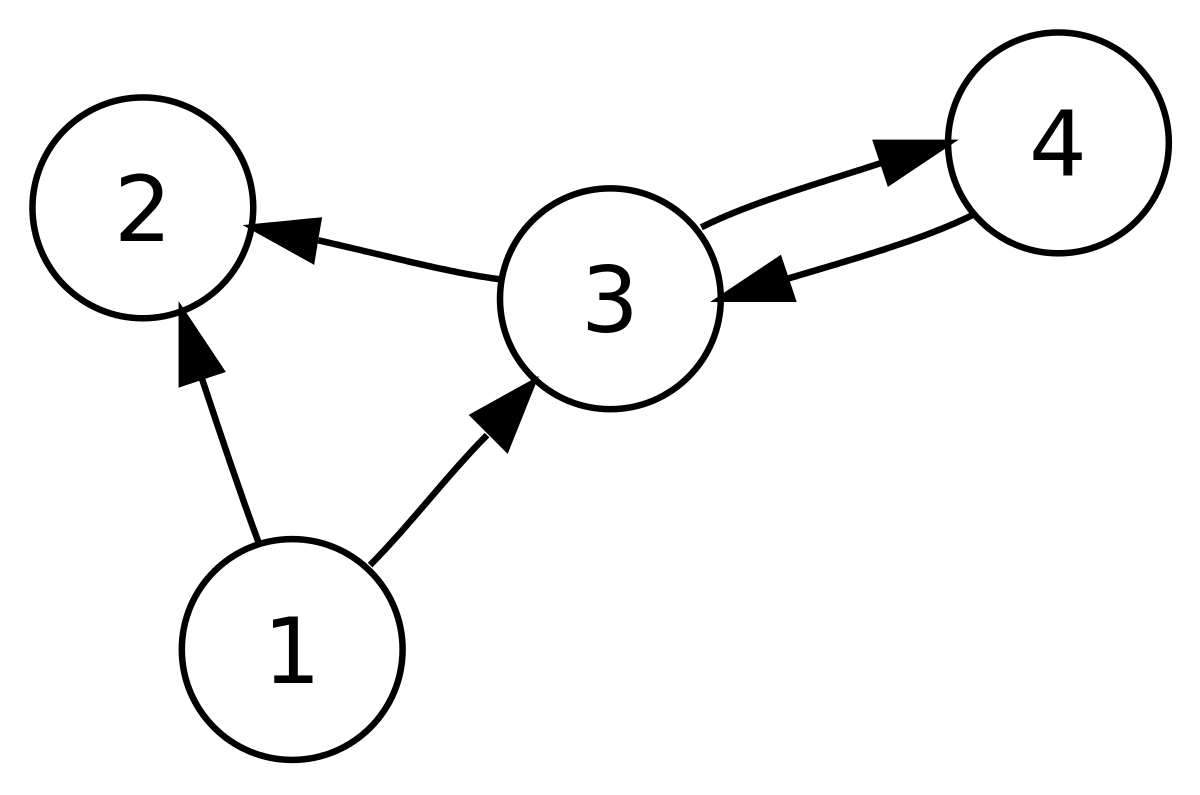
\includegraphics[scale=0.1]{graph}
    \\
        Figure 1.2: Directed Graph Overview
\end{center}

\section{Temporal Networks}
Temporal networks or dynamic networks are complex systems that change over time. Studying temporal networks fills the gap between network science and time-series analysis area\cite{HOLME201297}. 
This necessity of introducing the temporal aspect comes from the fact that nearly everything in the world is time-related, especially complex networks. From social networks to biological phenomena mostly, everything that is considered a complex system is subject to somewhat evolution over time\cite{PMID:35538294}. 
Social interactions are the clearest example, as new friendships might be introduced or cancelled, and the possibility of social interactions through the Internet has eased that by a lot.

\subsection{Dynamic Edge Set}
\label{sec:dygraphs}
As mentioned before a network can be thought of as a graph. In Dynamic networks, the Edge set can vary over time meaning every single interaction happens at a time T, which comes in as an Extra parameter for the edges. This means that Edges are identified now by a 3-tuple (source, destination, time). To give a better representation of a dynamic network edges can be grouped by discrete time so that every interaction in a time group W happens at that specific time, or inside that specific time window. After that groups are sorted by time and for each of them a static graph is created, with every Node of the network but only the Edges belonging to that group. Confronting each of those static graphs in order of time evolution gives an easy ad precise overview of the changes that the network has been through during the course of time.

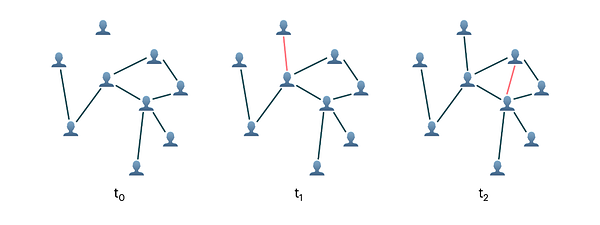
\includegraphics[scale=0.8]{temporalnetwork}

\begin{center}
    Figure 1.3: Temporal Network Change Overview
\end{center}

Isolated Nodes can be seen as “offline” users, while connected Nodes can be seen as “online” users interacting with some other online user(s) at that specific time. 

\subsection{Graph Concepts Adaptation}
\label{sec:dygraphs2}
The study of temporal networks is extremely important to have a better representation of the real-world systems that change throughout time. However, new challenges are brought up by the fact that introducing temporal networks adds one dimension to the data, making it not only harder to manage but also completely impacting even the basic notions of graphs. Every concept needs to be adapted when dealing with temporal networks. New algorithm design is then needed, with some problems being natural extensions of static graph problems to a temporal perspective and others being new problems being risen by the temporal evolution aspect. 
Not only the basic system structure but also the common concepts like node degree and adjacency now assume different values based on the discrete-time we are considering. On static unweighted graphs, a node degree is defined as the number of edges incident to that node and indicates both the total number of interactions and the number of nodes the node interacts with. Temporal networks allow for multiple Edges between the same pair of Nodes, similar to multi-graphs and weighted graphs, marking a clear distinction between the number of total interactions and the number of users interacted with. Reachability and path finding are now crucially related to the edges' effective presence at a discrete time and most importantly to their overall ordering, as shown in studies by Huanhuan Wu et. al about fath finding in temporal graphs.
\cite{10.14778/2732939.2732945}

\section{Social networks}
\label{sec:socialnetworks}
Social networks are large scale online networks that have become extremely powerful tools thanks to their ability to connect people and link disconnected networks together. They also allow for easier, effective and multiple interactions between people. This makes data flow very well through a social network thanks to the propagation that comes with interaction between the users in the form of ”word-of-mouth” communications. Information can flow in different ways through a social network, either through conversations between users and also through each user's feed, that depends on the user's following/friendship users set. Notice how simple directed temporal graphs can be used to model a social conversation network, whilst for interactions between multiple users it is needed to introduce higher order structures such as hypergraphs, that can better represent social networks adding group dynamics. However that increases the complexity of the data, so this work is limited to dual users conversations network, that can still provide a good amount of information spread, expecially through fast spreading informations like rumors\cite{10.2307/45018860}.

